\documentclass{article}%
\usepackage[T1]{fontenc}%
\usepackage[utf8]{inputenc}%
\usepackage{lmodern}%
\usepackage{textcomp}%
\usepackage{lastpage}%
\usepackage{authblk}%
\usepackage{graphicx}%
%
\title{Low titre autoantibodies against recoverin in sera of patients with small cell lung cancer but without a loss of vision}%
\author{Robert Potts}%
\affil{Division of Oncology/Hematology, Department of Internal Medicine, Korea University College of Medicine, Seoul, Republic of Korea, Division of Oncology/Hematology, Department of Pathology, Korea University College of Medicine, Seoul, Republic of Korea, Division of Oncology/Hematology, Department of Radiology, Korea University College of Medicine, Seoul, Republic of Korea, Division of Oncology/Hematology, Department of Surgery, Korea University College of Medicine, Seoul, Republic of Korea, Department of Physiology, College of Medicine, Hanyang University, Seoul, Republic of Korea}%
\date{01{-}01{-}2011}%
%
\begin{document}%
\normalsize%
\maketitle%
\section{Abstract}%
\label{sec:Abstract}%
Science is coming together on an amazing and revolutionary research program that will hopefully change the treatment of blood disorders.\newline%
{-}Dr. Frank Battaglia\newline%
It's called Protein Kinase LegK2. If this antibody or transducer program turns out to be the way to go in treating cancer, it could have a tremendous impact on the quality of life for millions of people around the world.\newline%
{-}Dr. Bruce Baroney\newline%
Most of us know what protein we eat and how it impacts our bodies. But what we don't know is that we tend to overeat during the middle of the night, run our mouths agape or even knock back too many drinks in an attempt to deflate our weight.\newline%
"Some of the strongest research on cell metabolism is that cell metabolism plays a great role in blood development," says Dr. Bruce Baroney, director of the La Jolla Blood Bank Research Institute.\newline%
Research by Baroney and his team has shown that a protein called protein legK2 is the most potent antibody in the body to modify a cell metabolism mechanism called Endoplasmic Reticulum Recruitment and Intracellular Replication (ERRIS). Without ERRIS, disease happens faster, as it should.\newline%
{-}Dr. Bruce Baroney\newline%
"While we know that protein legK2 is significantly active in ERRIS and our mice, we can't tell what it does in other cells," says Baroney.\newline%
Baroney and his research team hope to find out.\newline%
There are three phases of an ERRIS system. The first is REFRESH and it is lethal. The second stage is RESPONSE and it prevents ERRIS from becoming deadly. The third stage is ATTACK and it inhibits the ERRIS pathway.\newline%
The researchers at San Diego's La Jolla Blood Bank are at the forefront of developing the solution to prevent ERRIS from being dangerous.\newline%
"It stops severe, life{-}threatening, cancerous changes that can develop in a cell," says Baroney.

%
\subsection{Image Analysis}%
\label{subsec:ImageAnalysis}%


\begin{figure}[h!]%
\centering%
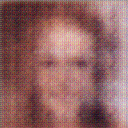
\includegraphics[width=150px]{500_fake_images/samples_5_159.png}%
\caption{A Man In A Suit And Tie Holding A Teddy Bear}%
\end{figure}

%
\end{document}